\documentclass[10pt, a4paper, oneside, headinclude,footinclude]{scrartcl}

\usepackage[nochapters, beramono, eulermath, pdfspacing, dottedtoc]{classicthesis} 
\usepackage{arsclassica} 
\usepackage[T1]{fontenc} 
\usepackage[utf8]{inputenc} 
\usepackage{graphicx} 

\graphicspath{{Figures/}}

\usepackage{enumitem} 
\usepackage{subfig} 
\usepackage{amsmath,amssymb,amsthm} 
\usepackage{lipsum} 
\usepackage{varioref} 

%%%%%%%%%%%%%%%%%%%%%%%%%%%%%%%%%%%%%%%%%%%%%%%%%%%%%%%%%%%%%%%%%%%%%%%%%%%%%%%%%%%%%%%%%%%%%%%%%%%%%%%%%%%

% SETTINGS DOCUMENT

%%%%%%%%%%%%%%%%%%%%%%%%%%%%%%%%%%%%%%%%%%%%%%%%%%%%%%%%%%%%%%%%%%%%%%%%%%%%%%%%%%%%%%%%%%%%%%%%%%%%%%%%%%%

\setcounter{tocdepth}{2} 
\renewcommand{\refname}{\spacedlowsmallcaps{References}} % For modifying the bibliography heading
\bibliographystyle{unsrt}


    %   THEOREM STYLES

\theoremstyle{definition} % Define theorem styles here based on the definition style (used for definitions and examples)
\newtheorem{definition}{Definition}
\theoremstyle{plain} 
\newtheorem{theorem}{Theorem}
\theoremstyle{remark} % Define theorem styles here based on the remark style (used for remarks and notes)

    %   HYPERLINKS

\hypersetup{
colorlinks=true, breaklinks=true, bookmarks=true,bookmarksnumbered,
urlcolor=webbrown, linkcolor=RoyalBlue, citecolor=webgreen, % Link colors
pdftitle={}, % PDF title
pdfauthor={\textcopyright}, % PDF Author
pdfsubject={}, % PDF Subject
pdfkeywords={}, % PDF Keywords
pdfcreator={pdfLaTeX}, % PDF Creator
pdfproducer={LaTeX with hyperref and ClassicThesis} % PDF producer
}
\hyphenation{Fortran hy-phen-ation} 

    %	TITLE AND AUTHOR(S)

\title{\normalfont\spacedallcaps{Article Title}} % The article title
\author{\spacedlowsmallcaps{Ali Ul Haq\textsuperscript{1}}} % The article author(s) - author affiliations need to be specified in the AUTHOR AFFILIATIONS block
\date{Month XXth 20XX} % An optional date to appear under the author(s)

%%%%%%%%%%%%%%%%%%%%%%%%%%%%%%%%%%%%%%%%%%%%%%%%%%%%%%%%%%%%%%%%%%%%%%%%%%%%%%%%%%%%%%%%%%%%%%%%%%%%%%%%%%%

% DOCUMENT START

%%%%%%%%%%%%%%%%%%%%%%%%%%%%%%%%%%%%%%%%%%%%%%%%%%%%%%%%%%%%%%%%%%%%%%%%%%%%%%%%%%%%%%%%%%%%%%%%%%%%%%%%%%%

\begin{document}


\renewcommand{\sectionmark}[1]{\markright{\spacedlowsmallcaps{#1}}} 
\lehead{\mbox{\llap{\small\thepage\kern1em\color{halfgray} \vline}\color{halfgray}\hspace{0.5em}\rightmark\hfil}} % The header style

\pagestyle{scrheadings} 
\maketitle 
\tableofcontents 
\section*{Abstract} 

\section{Problem 1: Design critique}

An short critique will be written for the Confluence visualisation by Harshawardhan Nene and Kedar Vaidya\footnote{\url{http://iibh.apphb.com/}}\\

The visualisations will be critiqued against the following points also shown in appendix 1

\begin{enumerate}[noitemsep]
    \item What is the problem domain or context of the visualisation?
    \item Which tasks can be achieved with this visualisation
    \item Consider Tufte\'s principles of graphical integrity
    \item Which of Tufte\'s visualisation design principles are adhered
    \item Describe how graphic design principles are used
    \item Comment on the visual encodings that are used
    \item Comment on subjective dimensions
    \item What is the intended goal of the visualization and is it achieved?
    \item Are there any things you would do differently, and why?
\end{enumerate}

\paragraph{1}\mbox{}\\
This visualisation visualises the differences of opinion between the audience and critics and attempts to map the financial succes of a movie to its ratings.

\paragraph{2}\mbox{}\\
The following tasks can be achieved:

\begin{itemize}[noitemsep]
    \item Find a correlation between high approval ratings from critics and the audience to the financial success.
    \item Relate if the critics are being over critical regarding different rating given by the audience.
    \item Find out if there is a relation between high financial budeting and high rating.
\end{itemize}

\paragraph{3}\mbox{}\\
The scale of the visualisation is unlabeled and there is no given legend to understand what the colors mean.\\ Furthermore there is no horizontal dimensions regarding in which year the movies are released.\\
There is not a significant lie factor due to the fact that there is sufficient separation between the user and critic rating and illustrates if the rating overlap or is significantly separated.

\paragraph{4}\mbox{}\\
When the option for fan art is disabled there still exist a high data ink ratio, meaning that there is a lot of data shown but for that data needs a lot of ink. Furthermore only one movie can be chosen. There is barely any chart junk and there exists a high data density.

\paragraph{5}\mbox{}\\
In this visualisation the contrast is used to show the differentiation between ratings. Due to the fact the same color is used for every movie there may exist a high repetition.\\
The data is closely shown and there also exists overlapping for some movies.

\paragraph{6}\mbox{}\\
The visual codings which is used primarily is color value and size. The color value is used to show the different ratings given by critics and the audience. The size is used to visualize the financial success. 

\paragraph{7}\mbox{}\\
Regarding the aesthetics,style,playfullness and vividness I would say that this visualisation is pretty dull and does not show a lot of variation.

\paragraph{8}\mbox{}\\
The intended goal was probably to provide the reader information about the discrepancy between critic rating and audience rating. In my opinion it is achieved but it is not clear immediatly.

\paragraph{9}\mbox{}\\
I would change the way the movie is represented and show it more along the lines of financial success, with an option to filter it through different genres. When the movie is clicked upon it may show the difference between audience and critics rating. Furthermore I would set the movies in chronological order of release.


\newpage
\section{Problem 2: Rainbow color map}
This figure shows the world elevation found on \url{https://commons.wikimedia.org/wiki/File:Elevation.jpg}. This visualisation\'s purpose is to inform about to world height difference and may be aimed for people interested in typography, flight planing, mountain climbing. It does not fail to convey the information and shows a difference between the elevation due to the fact that its represents the height different with a texture and more warmer color. The rainbow color in this case does not represent a clear visualisation in my opinion. This is because the color red and green have no added value regarding the elevation difference. Furthermore in this case the map gives of a \'loud\' feeling.


\begin{figure}[!htb]
    \centering
    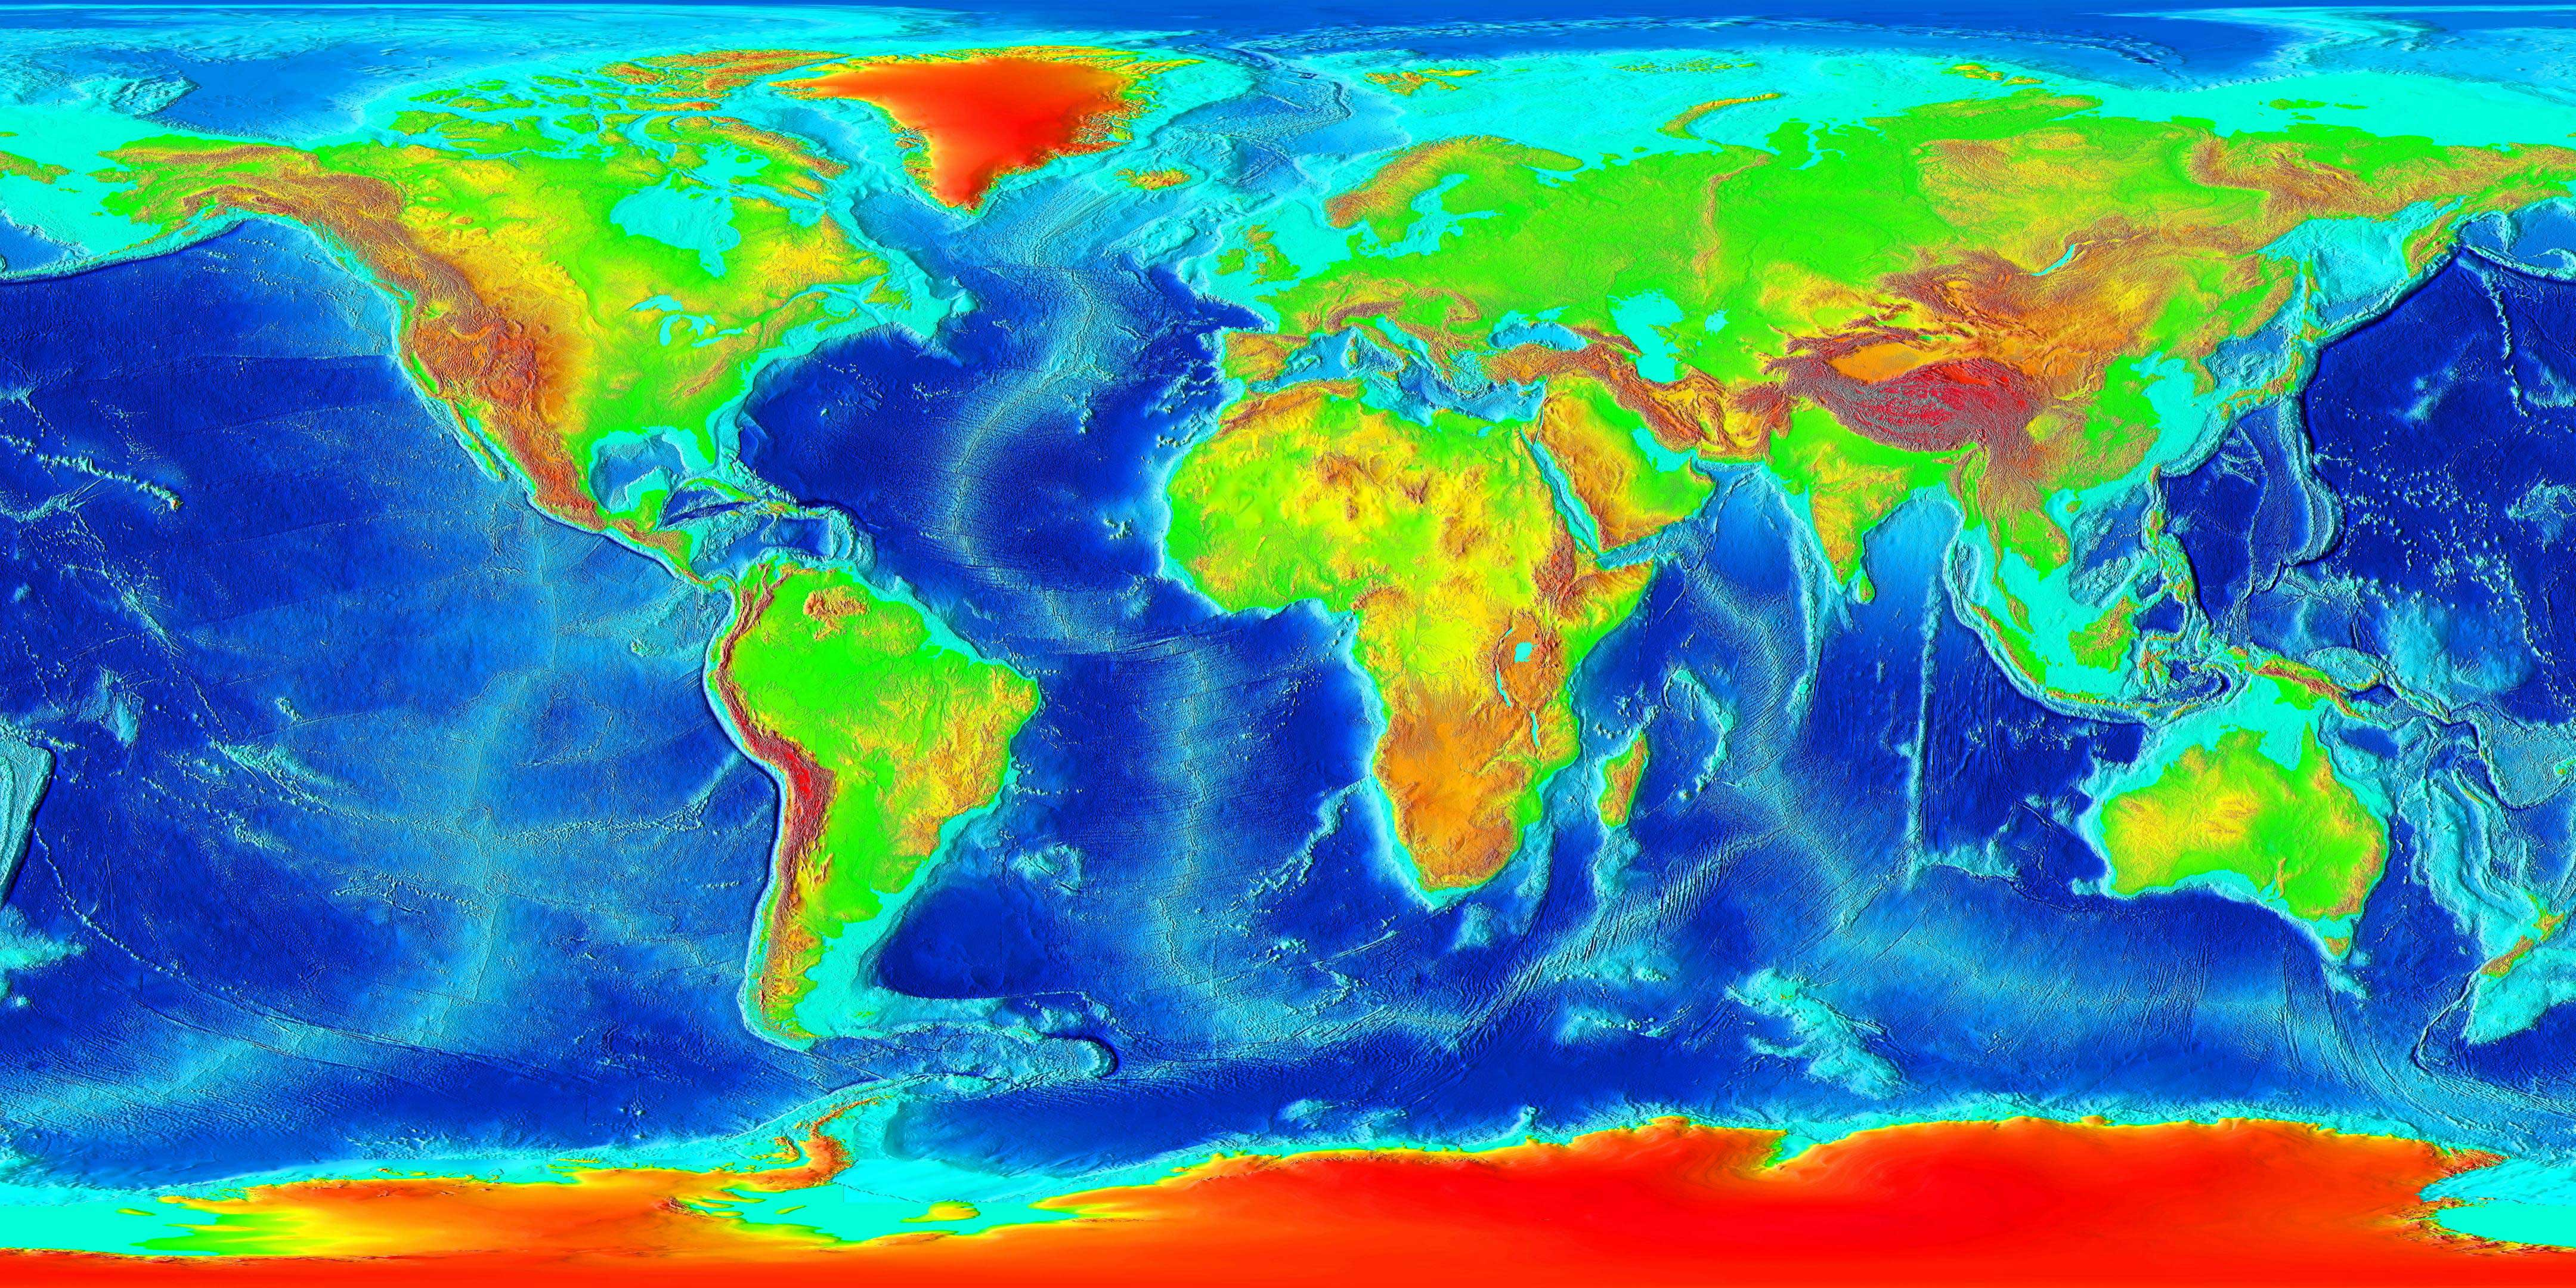
\includegraphics[width=\linewidth]{Figures/Elevation.jpg}
    \caption{World elevation map}
    \label{fig:elev}
\end{figure}
\section{Appendix 1}

\begin{itemize}[noitemsep]
    \item What is the problem domain or context of the visualization under consideration?
    \item Which tasks can be achieved with this visualization?
    \item Tufte’s principles of graphical integrity:
        \begin{itemize}[noitemsep]
            \item Are the scales appropriately labeled?
            \item Is the Lie factor high?
            \item Does the visualization show data variation and not design variation?
        \end{itemize}
    \item Tufte’s visualization design principles, are they adhered to?
        \begin{itemize}[noitemsep]
            \item Maximize the data-ink ratio.
            \item Avoid chart junk.
            \item Increase data density.
            \item Layer information.
        \end{itemize}
    \item Graphic design principles:
        \begin{itemize}[noitemsep]
            \item How is contrast used? What kind of contrast is used?
            \item How is repetition used?
            \item How is alignment used?
            \item How is proximity used?
        \end{itemize}
    \item Comment on the visual encodings that are used.
        \begin{itemize}[noitemsep]
            \item Which visual encodings are used?
            \item Are the visual encodings appropriate?
        \end{itemize}
    \item Comment on subjective dimensions such as aesthetics, style, playfulness
    and vividness.
    \item What is the intended goal of the visualization and is that goal achieved?
    \item Are there any things you would do differently, and why?
\end{itemize}


\bibliographystyle{unsrt}
\bibliography{bibliography.bib} % The file containing the bibliography

%----------------------------------------------------------------------------------------

\end{document}